\documentclass{article}
\renewcommand{\rmdefault}{psbx}
\usepackage[utf8]{inputenc}
\usepackage[T1]{fontenc}
\usepackage{textcomp}
\usepackage{eulervm}
\usepackage{amsmath}
\usepackage{amssymb}

\setlength{\textwidth}{160mm}
\setlength{\oddsidemargin}{0mm}
\setlength{\parindent}{0 mm}

\newcommand{\bfa}{{\bf a}}
\newcommand{\bfb}{{\bf b}}
\newcommand{\bfm}{{\bf m}}
\newcommand{\bfs}{{\bf s}}
\newcommand{\bfz}{{\bf z}}
\newcommand{\E}{{\mathbb E}}
\newcommand{\V}{{\mathbb V}}

\usepackage{tikz}
\usetikzlibrary{arrows,shapes,backgrounds,patterns,fadings,decorations.pathreplacing,decorations.pathmorphing}
\tikzset{>=stealth'}

\title{Cart and Double Pendulum Dynamics}
\author{Carl Edward Rasmussen}
% Edited by Jonas Umlauft 2014-07-16
\date{July 1st 2014}

\begin{document}

\maketitle

The cart and double pendulum dynamical system consists of a cart with
mass $m_1$ and an attached double pendulum. The double pendulum
consists of two pieces, the first of mass $m_2$ and length $\ell_2$
and the second has mass $m_3$ and length $\ell_3$. Both joints are
frictionless and unactuated, the double pendulum can move freely in the
vertical plane. The goal position is balancing the double pendulum vertically
above $x=0$, and the discrepancy is the distance $d$. The system is
actuated by applying a force $u$ horizontally to the cart. The state
of the system is given by the horizontal position of the cart $x_1$,
the two angles $\theta_2$ and $\theta_3$ (both measured anti-clockwise from
vertically up) and the time derivatives of these three variables,
$\dot x_1$, $\dot\theta_2$ and $\dot\theta_3$.

\begin{center}
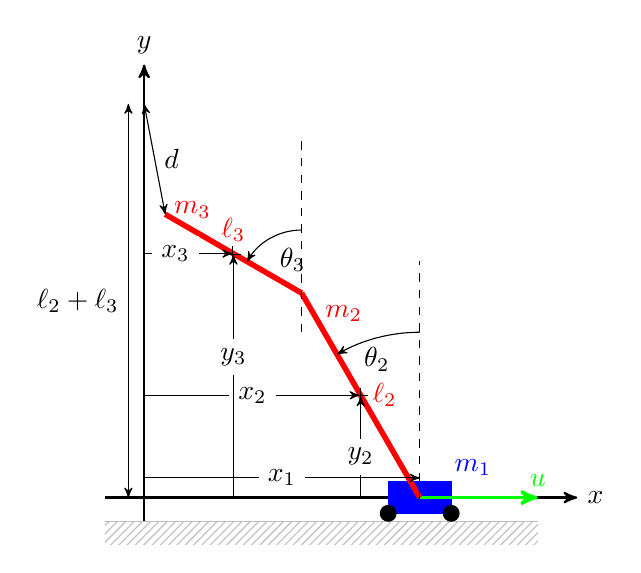
\begin{tikzpicture}

\def\lTwo{3}
\def\lThree{2}
\def\xOne{3.5} 
\def\thetaTwo {30}
\def\thetaThree {60}
\def\cartH {0.2}
\def\cartW {0.4}
\def\wheelR {0.1}

\pgfmathsetmacro{\xTwoThree}{\xOne - \lTwo*sin(\thetaTwo)}
\pgfmathsetmacro{\yTwoThree}{\lTwo*cos(\thetaTwo)}
\pgfmathsetmacro{\xTwo}{\xOne - 0.5*\lTwo*sin(\thetaTwo)}
\pgfmathsetmacro{\yTwo}{0.5*\lTwo*cos(\thetaTwo)}
\pgfmathsetmacro{\xThree}{\xOne - \lTwo*sin(\thetaTwo) - 0.5*\lThree*sin(\thetaThree)}
\pgfmathsetmacro{\yThree}{\lTwo*cos(\thetaTwo) + 0.5*\lThree*cos(\thetaThree)}
\pgfmathsetmacro{\xFour}{\xOne - \lTwo*sin(\thetaTwo) - \lThree*sin(\thetaThree)}
\pgfmathsetmacro{\yFour}{\lTwo*cos(\thetaTwo) + \lThree*cos(\thetaThree)}
\pgfmathsetmacro{\xTarget}{0}
\pgfmathsetmacro{\yTarget}{\lTwo +\lThree}

% coordinate system
\draw[thick,->] (0,-0.3) -- (0,\yTarget+0.5) node[anchor = south] {$y$};
\draw[thick,->] (-0.5,0) -- (\xOne+2,0) node[anchor = west] {$x$};
% rail:
\draw[draw=none,pattern=north east lines,pattern color=lightgray](-0.5,-\wheelR-\cartH) rectangle (5,-\wheelR-\cartH-0.3);
\draw[draw=lightgray] (-0.5,-\wheelR-\cartH) -- (5,-\wheelR-\cartH);
% cart:
\draw[draw=blue,fill=blue] (\xOne-\cartW,-\cartH) rectangle (\xOne+\cartW,\cartH) node[pos = 0.9, anchor = south west,blue] {$m_1$};  
\draw[draw=black,fill=black] (\xOne-\cartW,-\cartH) circle (\wheelR);
\draw[draw=black,fill=black] (\xOne+\cartW,-\cartH) circle (\wheelR);
\draw[very thick,draw=green,->] (\xOne,0) -- (\xOne+1.5,0) node[anchor=south,green] {$u$};
% pendulum:
\draw[line width = 2pt,red] (\xOne,0) -- (\xTwoThree,\yTwoThree) node[midway,anchor = west] {$\ell_2$} node[pos=0.9 ,anchor =  west]  {$m_2$};
\draw[line width = 2pt,red] (\xTwoThree,\yTwoThree) -- (\xFour,\yFour) node[midway,anchor =  south] {$\ell_3$} node[pos=0.8 ,anchor =  south]  {$m_3$};
\draw[dashed] (\xOne,0) -- (\xOne,\lTwo);
\draw[,->]([shift=(90:0.7*\lTwo)]\xOne,0) arc (90:90+\thetaTwo:0.7*\lTwo) node[anchor=north,midway] {$\theta_2$};
\draw[dashed] (\xTwoThree,\yTwoThree-0.5) -- (\xTwoThree,\yTwoThree+\lThree);
\draw[,->]([shift=(90:0.4*\lThree)]\xTwoThree,\yTwoThree) arc (90:90+\thetaThree:0.4*\lThree) node[anchor=north west,midway] {$\theta_3$};
% geometry:
\draw [<->] (\xTarget,\yTarget) -- (\xFour,\yFour) node[midway,anchor=  west] {$d$};
\draw [<->] (0-0.2,0) -- (\xTarget-0.2,\yTarget) node[midway,anchor=  east] {$\ell_2 + \ell_3$};
\draw [->,draw=black] (0,\cartH+0.05) -- (\xOne,\cartH+0.05) node[fill=white,midway]  {$x_1$};
\draw [->|,draw=black] (0,\yTwo) -- (\xTwo,\yTwo) node[fill=white, midway] {$x_2$};
\draw [->|,draw=black] (\xTwo,0) -- (\xTwo,\yTwo) node[fill=white, pos = 0.4] {$y_2$};
\draw [->|,draw=black] (0,\yThree) -- (\xThree,\yThree) node[fill=white, pos= 0.35] {$x_3$};
\draw [->|,draw=black] (\xThree,0) -- (\xThree,\yThree) node[fill=white, midway, anchor=south] {$y_3$};

\end{tikzpicture}  
\end{center}

The cart can move horizontally, with an applied external force
$-20{\rm N}\leq u\leq 20{\rm N}$,
and coefficient of friction $b=0.1{\rm Ns/m}$. The other physical
values are $m_1=m_2=m_3=0.5{\rm kg}$ and
$\ell_2=\ell_3=0.6{\rm m}$ (doesn't correspond to figure). Thus, the moment of
inertia around the midpoint of each part of the pendulum is
$I_2=I_3=0.015{\rm kg\,m^2}$.

\subsection*{Equations of Motion}

The geometric relationships gives the following conditions for the
coordinates of the midpoint of the two penduli:
\begin{alignat}{3}
x_2\;&=\;x_1-\tfrac{1}{2}\ell_2\sin\theta_2,&\qquad 
y_2\;&=\;\tfrac{1}{2}\ell_2\cos\theta_2,\\
x_3\;&=\;x_1-\ell_2\sin\theta_2-\tfrac{1}{2}\ell_3\sin\theta_3,&\qquad
y_3\;&=\;\ell_2\cos\theta_2+\tfrac{1}{2}\ell_3\cos\theta_3.
\end{alignat}
The squared velocities of the centres of gravity are
\begin{alignat}{1}
v_1^2\;&=\;\dot x_1^2, \qquad
v_2^2\;=\;\dot x_1^2-\ell_2\dot x_1\dot\theta_2\cos\theta_2+\tfrac{1}{4}\ell_2^2\dot\theta_2^2,\\
v_3^2\;&=\;\dot x_1^2-2\ell_2\dot x_1\dot\theta_2\cos\theta_2-
\ell_3\dot x_1\dot\theta_3\cos\theta_3+\ell_2^2\dot\theta_2^2+
\tfrac{1}{4}\ell_3^2\dot\theta_3^2+\ell_2\ell_3\dot\theta_2\dot\theta_3\cos\theta_2\cos\theta_3.
\end{alignat}
The system Lagrangian is
\[
\begin{split}
L\;=&\;T-V\;=\;
\tfrac{1}{2}m_1v_1^2+\tfrac{1}{2}m_2v_2^2+\tfrac{1}{2}m_3v_3^2+
\tfrac{1}{2}I_2\dot\theta_2^2+\tfrac{1}{2}I_3\dot\theta_3^2-m_2gy_2-m_3gy_3
\;\Rightarrow\\
L\;=&\;\tfrac{1}{2}(m_1+m_2+m_3)\dot x_1^2
-(\tfrac{1}{2}m_2+m_3)\ell_2\dot x_1\dot\theta_2\cos\theta_2 
+(\tfrac{1}{6}m_2+\tfrac{1}{2}m_3)\ell_2^2\dot\theta_2^2
-\tfrac{1}{2}m_3\ell_3\dot x_1\dot\theta_3\cos\theta_3+\\
&\;\tfrac{1}{6}m_3\ell_3^2\dot\theta_3^2
+\tfrac{1}{2}m_3\ell_2\ell_3\dot\theta_2\dot\theta_3\cos(\theta_2-\theta_3)
-(\tfrac{1}{2}m_2+m_3)g\ell_2\cos\theta_2-\tfrac{1}{2}m_3g\ell_3\cos\theta_3,
\end{split}
\]
where $g=9.82 {\rm m/s^2}$ is the accelleration of gravity.

The equations of motion are
\[
\frac{d}{dt}\frac{\partial L}{\partial\dot q_i}-\frac{\partial
  L}{\partial q_i}\;=\;Q_i,
\]
where $Q_i$ are the non-conservative forces. In our case
\begin{alignat}{1}
\frac{\partial L}{\partial\dot x_1}\;&=
\;(m_1+m_2+m_3)\dot x_1-(\tfrac{1}{2}m_2+m_3)\ell_2\dot\theta_2\cos\theta_2-\tfrac{1}{2}m_3\ell_3\dot\theta_3\cos\theta_3,\\
\frac{\partial L}{\partial x}\;&=\;0,\\
\frac{\partial L}{\partial\dot\theta_2}\;&=\;(\tfrac{1}{3}m_2+m_3)\ell_2^2\dot\theta_2 
-(\tfrac{1}{2}m_2+m_3)\ell_2\dot x_1\cos\theta_2+\tfrac{1}{2}m_3\ell_2\ell_3\dot\theta_3\cos(\theta_2-\theta_3),\\
\frac{\partial L}{\partial\theta_2}\;&=\;(\tfrac{1}{2}m_2+m_3)\ell_2(g+\dot x_1\dot\theta_2)\sin\theta_2-
\tfrac{1}{2}m_3\ell_2\ell_3\dot\theta_2\dot\theta_3\sin(\theta_2-\theta_3),\\
\frac{\partial L}{\partial\dot\theta_3}\;&=\;\tfrac{1}{3}m_3\ell_3^2\dot\theta_3 
-\tfrac{1}{2}m_3\ell_3\dot x_1\cos\theta_3+\tfrac{1}{2}m_3\ell_2\ell_3\dot\theta_2\cos(\theta_2-\theta_3),\\
\frac{\partial L}{\partial\theta_3}\;&=\;\tfrac{1}{2}m_3\ell_3(g+\dot x_1\dot\theta_3)\sin\theta_3+
\tfrac{1}{2}m_3\ell_2\ell_3\dot\theta_2\dot\theta_3\sin(\theta_2-\theta_3),
\end{alignat}
leading to the equations of motion
\[
\begin{split}
(m_1+m_2+m_3)\ddot x_1-(\tfrac{1}{2}m_2+m_3)\ell_2(\ddot\theta_2\cos\theta_2-\dot\theta_2^2\sin\theta_2)
-\tfrac{1}2m_3\ell_3(\ddot\theta_3\cos\theta_3-\dot\theta_3^2\sin\theta_3)\;=\;u-b\dot x_1,\\
(\tfrac{1}{3}m_2+m_3)\ell_2\ddot\theta_2-(\tfrac{1}{2}m_2+m_3)(\ddot x_1\cos\theta_2+g\sin\theta_2) 
+\tfrac{1}{2}m_3\ell_3[\ddot\theta_3\cos(\theta_2-\theta_3)+\dot\theta_3^2\sin(\theta_2-\theta_3)]\;=\;0,\\
\tfrac{1}{3}\ell_3\ddot\theta_3-\tfrac{1}{2}(\ddot x_1\cos\theta_3+g\sin\theta_3) 
+\tfrac{1}{2}\ell_2[\ddot\theta_2\cos(\theta_2-\theta_3)-\dot\theta_2^2\sin(\theta_2-\theta_3)]\;=\;0.
\end{split}
\]
Collecting the six state variables $\bfz=(\dot
x_1,\dot\theta_2,\dot\theta_3,x_1,\theta_2,\theta_3)$ the equations of motion can be conveniently
expressed as six coupled differential equations
\[
\frac{d\bfz}{dt}\;=\;\begin{array}{cc}A^{-1}&B\\I&0\end{array}
\]

\subsection*{Linearized Dynamics}

Linearizing the dynamics aroud the goal state, we can write the
following approximation
\[
\frac{d\bfz}{dt}\;\simeq\;q^{-1}(A\bfz+\bfb u),\qquad
q\;=\;2\ell_2\ell_3(m_1(4m_2+3m_3)+m_2(m_2+m_3)),\qquad
\bfb\;=\;\left[\!\begin{array}{c}
2\ell_2\ell_3(4m_2+3m_3)\\ 6\ell_3(2m_2+m_3)\\ -6\ell_2m_2\\ 0\\ 0\\ 0
\end{array}\!\right],
\]
 and
\[
A\;=\;\left[\!\begin{array}{cccccc}

-2\ell_2\ell_3(4m_2\!+\!3m_3)b&0&0&0&3\ell_2\ell_3(m_2+2m_3)(2m_2+m_3)g&-3\ell_2\ell_3m_2m_3g\\
-6\ell_3(2m_2+m_3)b&0&0&0&3\ell_3(m_2\!+\!2m_3)(4m_1\!+\!4m_2\!+\!m_3)g&-9\ell_3m_3(2m_1+m_2)g\\
6\ell_2m_2b&0&0&0&-9\ell_2(m_2+2m_3)(2m_1+m_2)g&\!\!\!3\ell_2(4m_1(m_2\!+\!3m_3)\!+\!m_2(m_2\!+\!4m_3))g\!\!\!\\
q&0&0&0&0&0\\
0&q&0&0&0&0\\
0&0&q&0&0&0\end{array}\!\right].
\]

\subsection*{Loss Function}

The instantaneous loss is given by
\[
F\;=\;1-\exp(-\frac{d^2}{2a^2}),
\]
were $d^2$ is the squared distance between the tip of the pendulum and
the point at distance $\ell_2 + \ell_3$ above the origin, and $a$ is the
\emph{width} parameter. Note that the instantaneous loss does not
depend on the speed variables, $\dot x_1,\ \dot\theta_2$ and $\dot\theta_3$. The
squared distance is
\[
d^2\;=\;(x_1-\ell_2\sin\theta_2-\ell_3\sin\theta_3)^2+(\ell-\ell_2\cos\theta_2+\ell_3\cos\theta_3)^2
\;=\;(\tilde\bfz-\mu)^\top Q(\tilde\bfz-\mu),
\]
where $\tilde\bfz$ is $\bfz$ augmented by four coordinates $\sin\theta_2, \sin\theta_3$ and
$\cos\theta_2, \cos\theta_3$ and
\[
Q\;=\;C^\top C,\quad
C\;=\;\begin{bmatrix}0& 0 & 0 & 1 & 0 & 0 & -\ell_1 & 0 & -\ell_2 & 0\\ 0&0& 0 & 0 & 0 & 0 & 0 & \ell_1 & 0 & \ell_2 \end{bmatrix},\quad
\mu\;=\;\begin{bmatrix}0&0&0&0&0&0&0&1&0&1\end{bmatrix}^\top.
\]
The \emph{expected loss}, averaging over the possibly uncertain states
is therefore
\[
\E[F(\tilde\bfz)]\;=\;1-\int F(\tilde\bfz)p(\tilde\bfz)d\tilde\bfz,
\]
which can be evaluated in closed form for Gaussian $p(\tilde\bfz)$, see
reward.pdf. Since the augmented state $\tilde\bfz$ will not generally
be Gaussian even if $\bfz$ is Gaussian, we project on to the closest
Gaussian by matching first and second moments.
\end{document}
 C = [1 0 0 0 0 0 -ell1 0 -ell2 0;
 0 0 0 0 0 0 0 ell1 0 ell2 ];

